\documentclass[journal,onecolumn,12pt]{IEEEtran}
\usepackage{graphicx}
\usepackage{caption}
\usepackage{listings}

\lstset{
  basicstyle=\scriptsize\tt,
}

\graphicspath{{figures/}}
\title{Unate Tautology}
\author{Nicholas Sica}

\begin{document}
\maketitle

\section{Report}
\begin{figure}
  \centering
  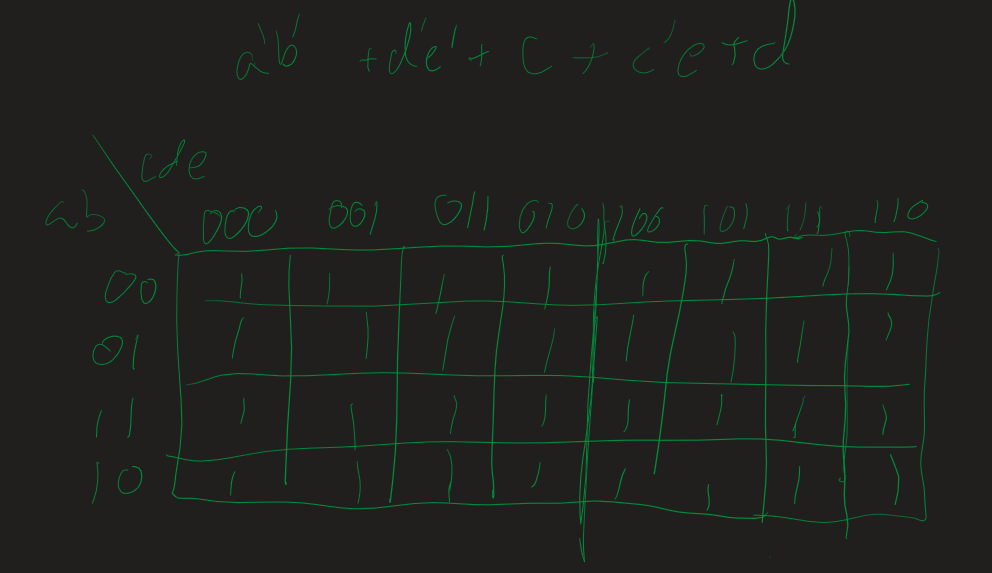
\includegraphics[width=0.95\columnwidth]{kmap_unate.png}
  \caption{A Karnaugh map of a unate problem}\label{fig:kmap_unate}
\end{figure}

\begin{figure}
  \centering
  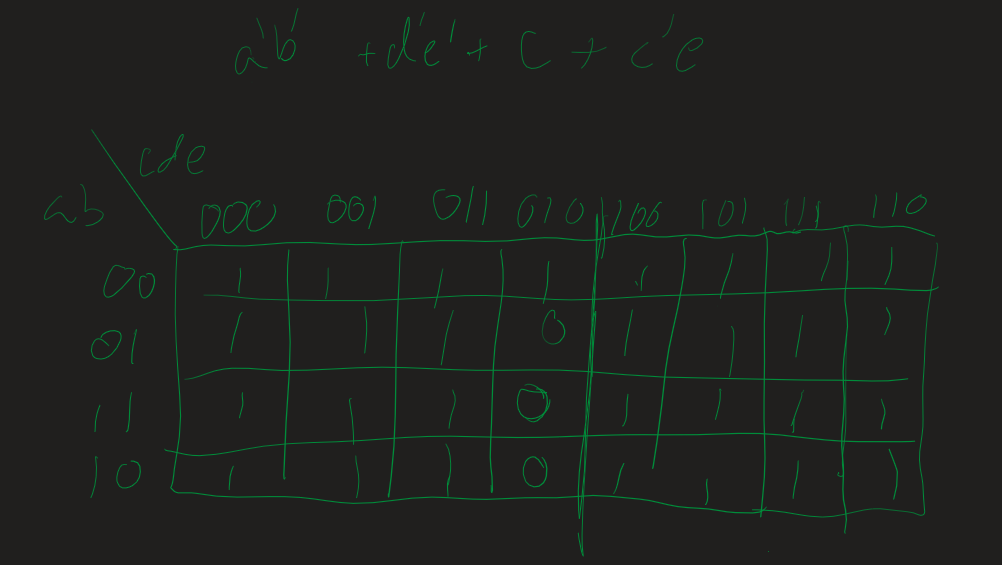
\includegraphics[width=0.95\columnwidth]{kmap_non_unate.png}
  \caption{A Karnaugh map of a non-unate problem}\label{fig:kmap_non_unate}
\end{figure}

This program was run on a linux operating system with Python
version 3.11.6. The program is invoked with ``python main.py
filename'', where the filename is the name of the input file to be
used. Most of the data structures are simple lists and flags to build up the cube list and the transposed cube list as well as whether the
structure is unate or has both polarities. The basic flow of the
program uses the pseudocode that was discussed in lecture as a
baseline and follows its layout.

Most of the solutions were double checked with Karnaugh maps and when there was some confusion,
walking through what should happen to debug the
program. In Fig~\ref{fig:kmap_unate}, the Karnaugh map for the unate
problem is shown and as expected, it is filled with true
outcomes. In Fig~\ref{fig:kmap_non_unate} the Karnaugh map for the
non-unate problem is shown and as expected, it is missing boxes with
true outcomes. The outputs for the previous two examples are in
Listing~\ref{lst:unate} and Listing~\ref{lst:non_unate}, respectively.
The output in Listing~\ref{lst:example_run} shows a run on the
example problem that was provided with the project. The entire program
is shown in Listing~\ref{lst:program}.

\lstinputlisting[caption=Unate output, label=lst:unate]{unate_output}
\lstinputlisting[caption=Non-unate output, label=lst:non_unate]{non_unate_output}
\lstinputlisting[caption=Project problem output, label=lst:example_run]{project_output}

\section{Program}
\lstinputlisting[caption=Unate tautology code, label=lst:program]{main.py}


\end{document}

%%% Local Variables:
%%% mode: latex
%%% TeX-master: t
%%% End:
